\documentclass[12pt]{article}

% ── Codificación y tipografía ──────────────────────────────────────────────────
\usepackage[utf8]{inputenc}
\usepackage[T1]{fontenc}
\usepackage{lmodern}
\usepackage{amssymb}
\usepackage[spanish,es-tabla]{babel}
\usepackage{microtype}

% ── Geometría ─────────────────────────────────────────────────────────────────
\usepackage[left=3cm, right=2.5cm, top=3cm, bottom=2.5cm]{geometry}
\setlength{\headheight}{24.02pt}
\addtolength{\topmargin}{-12.01pt}

% ── Gráficos y colores ────────────────────────────────────────────────────────
\usepackage{xcolor}
\usepackage{graphicx}
\usepackage{pgfgantt}
\usepackage{tikz}
\usetikzlibrary{shapes.geometric}

% ── Tablas ────────────────────────────────────────────────────────────────────
\usepackage{booktabs}
\usepackage{array}
\usepackage{multirow}
\usepackage{tabularx}
\usepackage{longtable}
\usepackage{colortbl}
\usepackage{makecell}

% ── Formato y estructura ──────────────────────────────────────────────────────
\usepackage{fancyhdr}
\usepackage{titlesec}
\usepackage{parskip}
\usepackage{enumitem}
\usepackage{hyperref}
\usepackage{amssymb}
\usepackage[htt]{hyphenat}
\usepackage{float}

% ── Paleta de colores ─────────────────────────────────────────────────────────
\definecolor{azulppal}{RGB}{0,70,127}
\definecolor{azulclaro}{RGB}{173,216,230}
\definecolor{grisoscuro}{RGB}{64,64,64}
\definecolor{grisclaro}{RGB}{245,245,245}
\definecolor{naranja}{RGB}{204,85,0}
\definecolor{verdeok}{RGB}{34,139,34}
\definecolor{g1}{RGB}{41,128,185}
\definecolor{g2}{RGB}{39,174,96}
\definecolor{g3}{RGB}{211,84,0}
\definecolor{g4}{RGB}{142,68,173}
\definecolor{g5}{RGB}{192,57,43}
\definecolor{tabhead}{RGB}{0,70,127}
\definecolor{tabrow}{RGB}{235,243,252}
\definecolor{rojoriesgo}{RGB}{180,30,30}
\definecolor{verdecumple}{RGB}{0,120,0}
\definecolor{amarillomed}{RGB}{180,140,0}

% ── hyperref ──────────────────────────────────────────────────────────────────
\hypersetup{
  colorlinks=true, linkcolor=azulppal, urlcolor=azulppal, citecolor=azulppal,
  pdftitle={Informe Técnico -- Capstone Analytics},
  pdfauthor={Sebastián Ramírez, Vicente Ramírez, Joaquín Parraud}
}

% ── Encabezado y pie ──────────────────────────────────────────────────────────
\pagestyle{fancy}
\fancyhf{}
\fancyhead[L]{\small\color{azulppal}\textbf{Informe Técnico -- Simulación Panadería de Supermercado}}
\fancyhead[R]{\small\color{grisoscuro}Mayo 2026}
\fancyfoot[C]{\small\thepage}
\renewcommand{\headrulewidth}{0.5pt}
\renewcommand{\headrule}{\hbox to\headwidth{\color{azulppal}\leaders\hrule height 0.5pt\hfill}}

% ── Secciones ─────────────────────────────────────────────────────────────────
\titleformat{\section}{\large\bfseries\color{azulppal}}{\thesection.}{0.5em}{}[\titlerule]
\titleformat{\subsection}{\normalsize\bfseries\color{grisoscuro}}{\thesubsection.}{0.5em}{}
\titleformat{\subsubsection}{\normalsize\itshape\color{grisoscuro}}{\thesubsubsection.}{0.5em}{}
\setlist[itemize]{topsep=2pt,itemsep=1pt,leftmargin=*}
\setlist[enumerate]{topsep=2pt,itemsep=1pt,leftmargin=*}
\setcounter{tocdepth}{2}



% ─────────────────────────────────────────────────────────────────────────────
\begin{document}
\pdfpagewidth=210mm
\pdfpageheight=297mm
\setlength{\parskip}{6pt}

% ══════════════════════════════════════════════════════════════════════════════
%  PORTADA
% ══════════════════════════════════════════════════════════════════════════════
\begin{titlepage}
\centering
\vspace*{0.4cm}

\includegraphics[width=0.36\linewidth]{../UDD.png}\\[0.9cm]
{\color{azulppal}\rule{\linewidth}{2.5pt}}\\[0.5em]
{\Huge\bfseries\color{azulppal} Informe Técnico}\\[0.4em]
{\large\bfseries\color{grisoscuro} Proyecto Capstone Analytics}\\[0.2em]
{\color{azulppal}\rule{\linewidth}{1pt}}\\[0.8em]
{\Large\itshape\color{grisoscuro}
  Simulación de Eventos Discretos:\\[0.3em]
  Proceso de Fabricación de Pan\\
  en Panadería de Supermercado}

\vspace{0.85cm}
\begin{tabular}{@{}ll@{}}
  \textbf{Universidad:}      & Universidad del Desarrollo \\[3pt]
  \textbf{Ramo:}             & Capstone Analytics \\[3pt]
  \textbf{Código:}           & IIC511AD \\[3pt]
  \textbf{Profesor:}         & Victor Vera, PhD \\[3pt]
  \textbf{Documento:}        & Proyecto de Simulación -- Informe Técnico \\[3pt]
  \textbf{Fecha:}            & 20 de mayo de 2026 \\[3pt]
\end{tabular}

\vfill
\begin{flushright}
{\small\color{grisoscuro}
\textbf{Integrantes}\\[4pt]
Joaquín Parraud\\
Sebastián Ramírez\\
Vicente Ramírez}
\end{flushright}
\vspace{0.4cm}
{\color{azulppal}\rule{\linewidth}{2.5pt}}\\[0.3em]
{\small\color{grisoscuro} Capstone Analytics IIC511AD -- Ingeniería Civil Industrial -- Universidad del Desarrollo}
\end{titlepage}

\tableofcontents

% ══════════════════════════════════════════════════════════════════════════════
\newpage
\section{Resumen ejecutivo}
% ══════════════════════════════════════════════════════════════════════════════

La panadería del supermercado enfrenta un déficit crítico de nivel de servicio: la configuración actual entrega solo un \textbf{68,3\%} de la demanda diaria, cuando el estándar mínimo exigido es el \textbf{95\%} para cada tipo de pan. En términos concretos, más de 2.500~kg de pan solicitado no llegan a la sala de ventas en un día típico --- pérdida directa de venta y deterioro de la experiencia de compra.

Este informe presenta los resultados del modelo de simulación de eventos discretos construido para identificar, con evidencia cuantitativa, qué combinación de recursos y política de producción cierra esa brecha.

\medskip
\noindent\textbf{Objetivo.} Determinar la configuración operacional que alcanza el 95\%~de demanda satisfecha para los diez tipos de pan, con el menor costo operativo posible.

\medskip
\noindent\textbf{Principales hallazgos.} Se evaluaron cinco escenarios:

\begin{table}[H]
\centering
\renewcommand{\arraystretch}{1.3}
\begin{tabularx}{\textwidth}{lXcc}
\toprule
\rowcolor{tabhead}
\color{white}\textbf{Escenario} & \color{white}\textbf{Descripción} &
\color{white}\textbf{\makecell{Nivel de\\servicio}} &
\color{white}\textbf{\makecell{¿Cumple\\95\%?}} \\
\midrule
\rowcolor{tabrow} Caso~0 & Configuración actual (2~panaderos, 1~manipulador, 1~horno) & 68,3\% & \textcolor{rojoriesgo}{\textbf{No}} \\
Caso~A & +1~panadero (3 total), política híbrida & 84,7\% & \textcolor{rojoriesgo}{\textbf{No}} \\
\rowcolor{tabrow} Caso~B & Caso~A $+$ 2.° horno & 79,1\% & \textcolor{rojoriesgo}{\textbf{No}} \\
Caso~C & Caso~B $+$ compartir estaciones & 79,3\% & \textcolor{rojoriesgo}{\textbf{No}} \\
\rowcolor{tabrow} Caso~D & Caso~A $+$ lotes óptimos (techo teórico, no implementable directo) & 98,6\% & \textcolor{naranja}{\textbf{Ref.}} \\
\bottomrule
\end{tabularx}
\end{table}

\medskip
\noindent\textbf{Hallazgo crítico.} Agregar un segundo horno \emph{sin} aumentar los panaderos y manipuladores empeora el sistema: el nivel baja de 84,7\% a 79,1\% (Caso~B). El horno no es el cuello de botella --- los panaderos sí.

\medskip
\noindent\textbf{Recomendación final.} Tres acciones secuenciales, sin inversión en equipamiento mayor:
\begin{enumerate}
  \item \textbf{Contratar 1 panadero adicional} (total 3). Impacto inmediato: $+16,4$~pp en nivel de servicio global.
  \item \textbf{Adelantar inicio de producción a las 04:00--05:00}. Permite completar ciclos adicionales antes del primer pico de demanda (12:00--14:00).
  \item \textbf{Agregar 1 manipulador} (total 2). Destraba la carga/descarga del horno y acelera la reposición a sala.
\end{enumerate}

% ══════════════════════════════════════════════════════════════════════════════
\newpage
\section{Descripción del sistema}
% ══════════════════════════════════════════════════════════════════════════════

\subsection{Contexto operacional}

La panadería es una unidad de producción interna de un supermercado. Su objetivo es abastecer la sala de autoservicio con pan fresco elaborado en el mismo local. La sala opera en horario de atención de público de \textbf{09:00 a 21:00 horas}, con producción que comienza antes de la apertura para garantizar disponibilidad desde el primer momento. El sistema produce \textbf{diez variedades de pan fresco} con una demanda total de \textbf{8.200~kg/día}, distribuida en un perfil horario con picos en 12:00--14:00 y 18:00--20:00. Cualquier demanda no satisfecha se pierde: el cliente no espera ni regresa por ese producto ese mismo día.

\subsection{Proceso productivo}

Cada variedad de pan recorre la misma secuencia de etapas, con tiempos específicos por producto: pesado y dosificación de ingredientes, mezclado (intervención manual del panadero más ciclo automático de mezcladora), amasado manual, reposo o fermentación en masa, dividido y formado, fermentación final, horneado en horno industrial, enfriamiento y reposición a sala.

\begin{figure}[H]
\centering
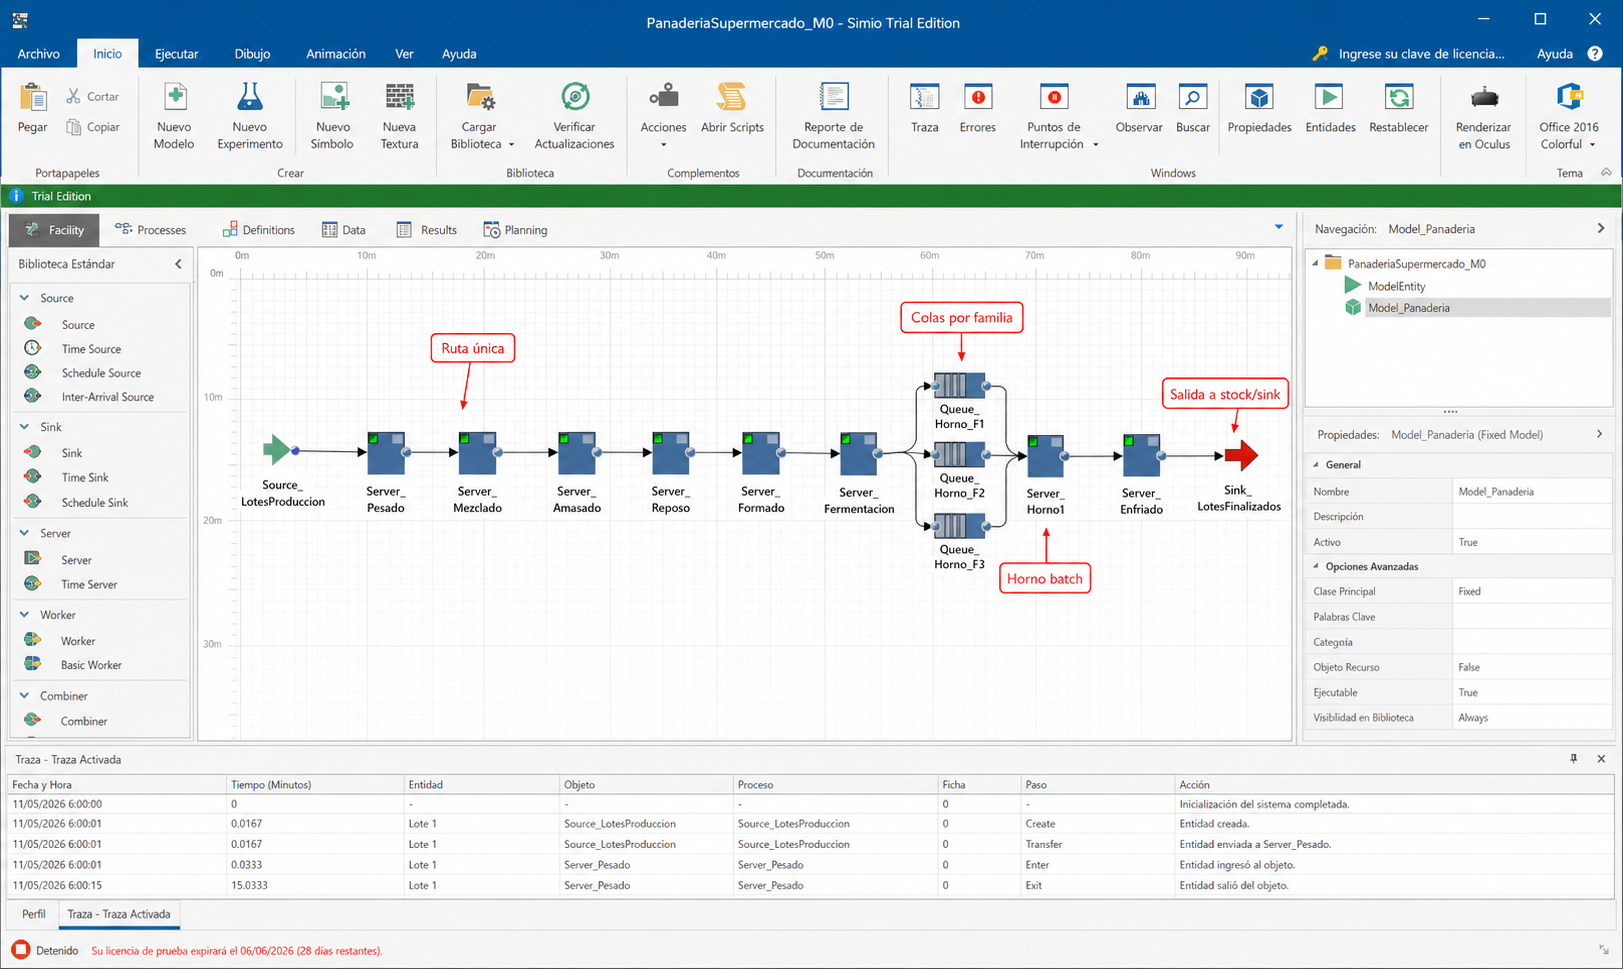
\includegraphics[width=0.85\linewidth]{../GuiaImplementacionSimio/figures_ai/ai_05_production_route.png}
\caption{Flujo del proceso productivo del pan: desde el pesado de ingredientes hasta la reposición a sala.}
\label{fig:ruta-tec}
\end{figure}

\subsection{Hornos batch}

Los hornos operan por \textbf{corridas completas} (modo \textit{batch}): se cargan, hornean y descargan en bloque antes de iniciar la siguiente corrida. Esto significa que el horno no puede recibir nuevos lotes mientras está en operación. Los diez tipos de pan se agrupan en tres familias según su temperatura y tiempo de cocción, y una corrida no puede mezclar familias. Los parámetros operativos del horno se resumen en la Tabla~\ref{tab:horno-tec}.

\begin{table}[H]
\centering
\caption{Parámetros operativos del horno batch}
\label{tab:horno-tec}
\renewcommand{\arraystretch}{1.3}
\begin{tabularx}{\textwidth}{lXc}
\toprule
\rowcolor{tabhead}
\color{white}\textbf{Parámetro} & \color{white}\textbf{Descripción} & \color{white}\textbf{Valor} \\
\midrule
\rowcolor{tabrow} Familia~1 (corto)  & Pan Hot Dog, Dobladita, Bocado de Dama & 14~min \\
Familia~2 (medio)                    & Marraqueta, Hallulla, Hallulla Integral, Amasado & 18~min \\
\rowcolor{tabrow} Familia~3 (largo)  & Marraqueta Integral, Ciabatta, Baguette & 21~min \\
Capacidad máxima                     & 6~carros $\times$ 18~bandejas & 108~bandejas \\
\rowcolor{tabrow} Carga mínima       & 50\% de capacidad & 600~kg \\
Espera máxima                        & Tiempo antes de disparar corrida & 15~min \\
\rowcolor{tabrow} Setup misma familia & Sin cambio de familia & 0~min \\
Setup distinta familia               & Cambio entre familias & 5~min \\
\rowcolor{tabrow} Carga/descarga     & Manipulador requerido & 5~min c/u \\
\bottomrule
\end{tabularx}
\end{table}

\begin{figure}[H]
\centering
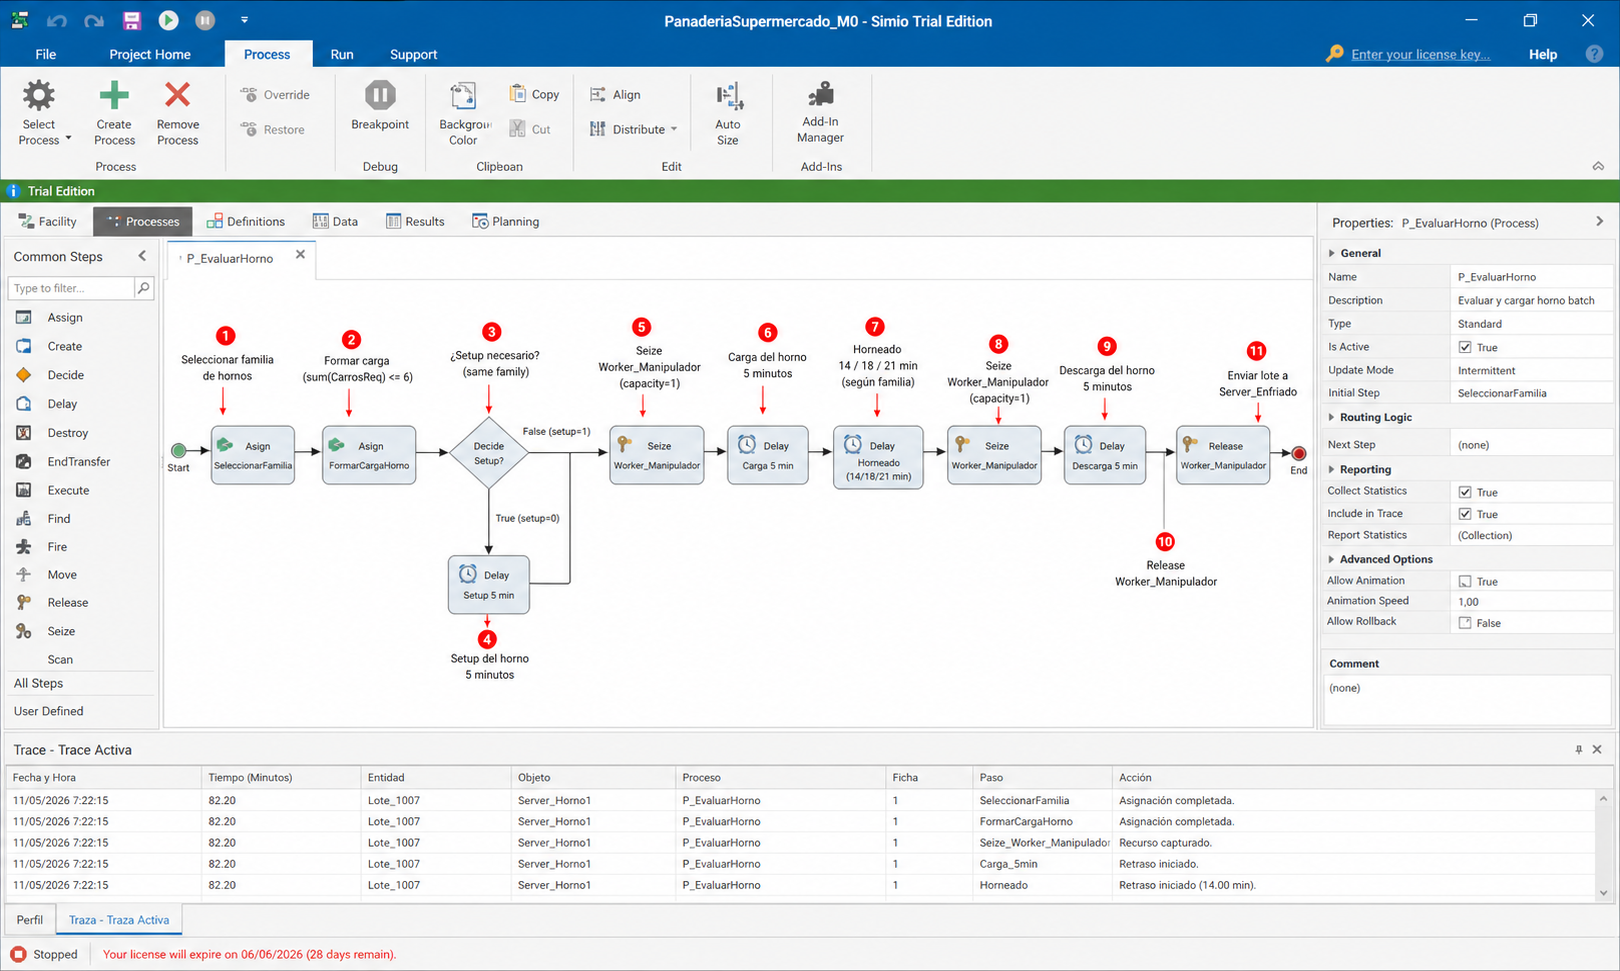
\includegraphics[width=0.85\linewidth]{../GuiaImplementacionSimio/figures_ai/ai_06_oven_batch_process.png}
\caption{Operación batch del horno: agrupación por familia de horneado, formación de carga por carros y restricción de no mezclar familias en una misma corrida.}
\label{fig:horno-tec-fig}
\end{figure}

\subsection{Demanda}

La demanda diaria total es 8.200~kg distribuidos en diez tipos de pan con perfiles horarios distintos. Cada cliente compra uno, dos o tres tipos de pan con probabilidades 50\%, 35\% y 15\% respectivamente, y la cantidad por tipo sigue una distribución triangular específica del producto (Tabla~\ref{tab:demanda-tec}).

\begin{table}[H]
\centering
\caption{Demanda diaria por tipo de pan y distribución de compra}
\label{tab:demanda-tec}
\renewcommand{\arraystretch}{1.3}
\begin{tabularx}{\textwidth}{Xccccc}
\toprule
\rowcolor{tabhead}
\color{white}\textbf{\makecell[c]{Tipo de\\pan}} &
\color{white}\textbf{Familia} &
\color{white}\textbf{\makecell[c]{Dem. diaria\\(kg)}} &
\color{white}\textbf{\makecell[c]{Mín.\\(kg)}} &
\color{white}\textbf{\makecell[c]{Moda\\(kg)}} &
\color{white}\textbf{\makecell[c]{Máx.\\(kg)}} \\
\midrule
\rowcolor{tabrow} Marraqueta            & 2 (18~min) & 2.000 & 0,25 & 0,75 & 2,0 \\
Hallulla                                & 2 (18~min) & 1.700 & 0,25 & 0,75 & 2,0 \\
\rowcolor{tabrow} Pan Hot Dog           & 1 (14~min) & 1.200 & 0,25 & 0,75 & 2,0 \\
Marraqueta Integral                     & 3 (21~min) &   800 & 0,25 & 0,75 & 2,0 \\
\rowcolor{tabrow} Hallulla Integral     & 2 (18~min) &   800 & 0,25 & 0,75 & 2,0 \\
Amasado                                 & 2 (18~min) &   380 & 0,25 & 0,75 & 2,0 \\
\rowcolor{tabrow} Ciabatta              & 3 (21~min) &   400 & 0,25 & 0,75 & 2,0 \\
Baguette                                & 3 (21~min) &   350 & 0,25 & 0,75 & 2,0 \\
\rowcolor{tabrow} Dobladita             & 1 (14~min) &   350 & 0,25 & 0,75 & 2,0 \\
Bocado de Dama                          & 1 (14~min) &   220 & 0,25 & 0,75 & 2,0 \\
\midrule
\rowcolor{tabrow}\multicolumn{2}{l}{\textbf{Total}} & \textbf{8.200} & & & \\
\bottomrule
\end{tabularx}
\end{table}

% ══════════════════════════════════════════════════════════════════════════════
\newpage
\section{Supuestos del modelo}
% ══════════════════════════════════════════════════════════════════════════════

Los supuestos que estructuran el modelo y sus resultados son los siguientes. El modelo representa la producción a \textbf{nivel de lote}: cada grupo de pan que entra al proceso es una unidad discreta de producción. El inventario se mide en \textbf{kilogramos} y los recursos (panaderos, manipuladores, hornos) se modelan como \textbf{capacidades discretas} que pueden estar ocupadas o libres. Las \textbf{variables de decisión} modeladas son: número de panaderos, número de manipuladores, número de hornos, hora de inicio de producción y política de secuenciamiento de lotes.

\begin{enumerate}
  \item La sala opera entre las 09:00 y las 21:00 horas; la producción comienza antes de la apertura para garantizar disponibilidad inicial.
  \item La demanda no satisfecha no se recupera: cada quiebre representa una pérdida directa de venta.
  \item Los hornos operan exclusivamente en modo batch por corrida completa; no se permite mezclar familias en una misma carga.
  \item Los panaderos y manipuladores trabajan en turnos con colaciones (45~min) y dos descansos de 15~min escalonados, de modo que ninguna función queda sin cobertura simultáneamente.
  \item No se modelan fallas de equipos ni mantenimiento mayor: se asume disponibilidad nominal de hornos, mezcladoras y amasadoras durante la jornada.
  \item El abastecimiento de materias primas se considera ilimitado dentro del horizonte diario.
  \item Los sobrantes al cierre del día no son objeto de optimización del modelo.
  \item La cantidad comprada por cliente por tipo de pan sigue una distribución triangular (mín. 0,25~kg, moda 0,75~kg, máx. 2,0~kg) --- supuesto uniforme para todos los productos por ausencia de datos de ticket POS.
  \item La probabilidad de comprar 1, 2 ó 3 tipos de pan en una visita es 50\%, 35\% y 15\% respectivamente --- supuesto de comportamiento sin datos transaccionales.
\end{enumerate}

% ══════════════════════════════════════════════════════════════════════════════
\newpage
\section{Enfoque de modelación}
% ══════════════════════════════════════════════════════════════════════════════

\subsection{Tipo de modelo}

El modelo es una simulación de eventos discretos con dos tipos de entidades en flujo: clientes que llegan a la sala según un perfil horario y consumen inventario, y lotes de producción que recorren la ruta productiva.

\subsection{Qué se modeló}

\begin{itemize}
  \item \textbf{Demanda:} llegada de clientes individuales según tasa horaria calibrada; cada cliente elige el número de productos a comprar y los tipos según las probabilidades horarias.
  \item \textbf{Inventario:} vector de stock por tipo de pan en la sala de ventas; cada compra descuenta el stock y los quiebres se registran como eventos.
  \item \textbf{Producción:} ruta única de etapas con tiempos parametrizados por producto, alimentada por una política de generación de lotes.
  \item \textbf{Horno:} tres grupos de productos (uno por familia de temperatura), formación de carga por carros y bandejas, política de preparación explícita entre familias.
  \item \textbf{Recursos humanos:} manipuladores con horarios y descansos explícitos; panaderos como capacidad lógica asignable a las etapas manuales.
  \item \textbf{Reposición:} traslado del pan desde enfriamiento hasta el inventario de sala, requiere manipulador.
\end{itemize}

\subsection{Qué no se modeló (fuera de alcance)}

Compras y gestión de materias primas, transporte externo, fallas de equipos, ventas de otros productos del supermercado, deterioro por sobreproducción, ni variaciones de precio.

\subsection{Parametrización de escenarios}

Todas las decisiones de escenario (número de panaderos, manipuladores, hornos; hora de inicio; política de secuenciamiento) se controlan desde una tabla centralizada de parámetros. La lógica del modelo no requiere modificación para cambiar de escenario.

\subsection{Parámetros cuantificados del modelo}

La Tabla~\ref{tab:parametros-modelo} detalla los parámetros del modelo con sus valores base y nivel de sensibilidad. Los parámetros provienen de la tabla \texttt{Tbl\_Supuestos}, que consolida todos los supuestos cuantitativos junto con su fuente y estado.

\begin{table}[H]
\centering
\caption{Parámetros del modelo: nombre, propósito y valor base}
\label{tab:parametros-modelo}
\renewcommand{\arraystretch}{1.3}
\begin{tabularx}{\textwidth}{lXcc}
\toprule
\rowcolor{tabhead}
\color{white}\textbf{Parámetro} &
\color{white}\textbf{Propósito en el modelo} &
\color{white}\textbf{Valor base} &
\color{white}\textbf{Sensib.} \\
\midrule
\rowcolor{tabrow}\texttt{MinKgCompra}            & Límite inferior de la distribución triangular de cantidad comprada por cliente por tipo de pan. Define el escenario de compra mínima posible. & 0,25~kg & Baja \\
\texttt{ModaKgCompra}           & Valor modal de la distribución triangular de cantidad comprada. Representa la compra más probable por tipo de pan. & 0,75~kg & Baja \\
\rowcolor{tabrow}\texttt{MaxKgCompra}            & Límite superior de la distribución triangular. Representa el máximo de compra en un único tipo de pan por visita. & 2,0~kg & Baja \\
\texttt{ProbCompra1Producto}    & Probabilidad de que un cliente elija exactamente 1 tipo de pan en su visita. & 0,50 & Media \\
\rowcolor{tabrow}\texttt{ProbCompra2Productos}   & Probabilidad de que un cliente elija 2 tipos distintos de pan en su visita. & 0,35 & Media \\
\texttt{ProbCompra3Productos}   & Probabilidad de que un cliente elija 3 tipos distintos de pan en su visita. & 0,15 & Media \\
\rowcolor{tabrow}\texttt{VelocidadPanadero}      & Velocidad de desplazamiento físico del panadero entre estaciones de trabajo. Afecta los tiempos de traslado. & 1,2~m/s & Baja \\
\texttt{VelocidadManipulador}   & Velocidad del manipulador al moverse con un carro cargado. Afecta el tiempo de traslado del pan al horno y a sala. & 0,8~m/s & Baja \\
\rowcolor{tabrow}\texttt{CargaMinKgBase}         & Carga mínima de kilogramos para disparar una corrida de horno. Si no se alcanza en \texttt{EsperaMaxMin}, la corrida se dispara igualmente. & 600~kg & Alta \\
\texttt{MaxCarrosHorno}         & Capacidad máxima del horno expresada en carros por corrida. Limita la cantidad total que puede hornearse simultáneamente. & 6~carros & Media \\
\rowcolor{tabrow}\texttt{EsperaMaxMin}           & Tiempo máximo de espera para formar una carga de horno antes de disparar la corrida aunque no se alcance la carga mínima. & 15~min & Media \\
\texttt{IntervaloLiberacionMin} & Intervalo de tiempo entre evaluaciones de producción push en la política \texttt{BASE\_HIBRIDA}. Define la frecuencia de generación proactiva de lotes. & 30~min & Media \\
\rowcolor{tabrow}\texttt{PuntoReposicionMin}     & Cobertura mínima de stock (en minutos de demanda) bajo la cual se dispara la reposición pull. & 45~min & Media \\
\texttt{CoberturaObjetivoMin}   & Cobertura de stock objetivo a alcanzar cuando se genera un lote push, expresada en minutos de demanda esperada. & 90~min & Media \\
\bottomrule
\end{tabularx}
\end{table}

\subsection{Variables de respuesta del modelo (tallies)}

Cada corrida del experimento registra las siguientes variables de respuesta por producto y por escenario:

\begin{table}[H]
\centering
\caption{Variables de respuesta registradas por el modelo}
\label{tab:tallies}
\renewcommand{\arraystretch}{1.3}
\begin{tabularx}{\textwidth}{lX}
\toprule
\rowcolor{tabhead}
\color{white}\textbf{Variable} &
\color{white}\textbf{Descripción y unidad} \\
\midrule
\rowcolor{tabrow}\texttt{nivel\_servicio\_pct}       & Porcentaje de demanda satisfecha: \texttt{demanda\_satisfecha\_kg / demanda\_total\_kg × 100}. KPI principal del estudio. Medido por producto y como total ponderado (\%). \\
\texttt{demanda\_total\_kg}          & Total de kilogramos demandados en el horizonte de simulación (09:00--21:00). Varía levemente entre réplicas por la estocasticidad de llegadas (kg). \\
\rowcolor{tabrow}\texttt{demanda\_satisfecha\_kg}    & Kilogramos de pan efectivamente entregados a clientes. Acumulado en \texttt{P\_ConsumirInventario} solo cuando hay stock disponible (kg). \\
\texttt{demanda\_perdida\_kg}        & Kilogramos de demanda no atendida: \texttt{demanda\_total\_kg - demanda\_satisfecha\_kg}. Representa la venta perdida directa (kg). \\
\rowcolor{tabrow}\texttt{stockout\_count}            & Número de eventos de quiebre: instancias en que un cliente solicitó un producto y el stock era $\leq 0$ en ese momento. Un stockout puede representar múltiples kg perdidos. \\
\texttt{lotes\_liberados\_total}     & Total de lotes de producción generados en el día por el modelo. Cada lote recorre la ruta completa (pesado → sala). \\
\rowcolor{tabrow}\texttt{lotes\_liberados\_push}     & Lotes generados por el mecanismo push periódico (interval timer \texttt{IntervaloLiberacionMin}). Refleja producción proactiva planificada. \\
\texttt{lotes\_liberados\_pull}      & Lotes generados por el mecanismo pull reactivo, activados cuando \texttt{P\_ConsumirInventario} detecta un quiebre. \\
\rowcolor{tabrow}\texttt{setup\_horno\_count}        & Número de cambios de familia registrados en el horno durante el día. Cada cambio de familia entre corridas consecutivas cuenta como un setup. \\
\texttt{tiempo\_setup\_total\_min}   & Tiempo total acumulado en setups de horno. Cada cambio de familia cuesta 5~min; cambios dentro de la misma familia cuestan 0~min (min). \\
\bottomrule
\end{tabularx}
\end{table}

\subsection{Procesos principales del modelo}

La lógica del modelo se implementa en ocho procesos con triggers explícitos. Cada entrada indica qué hace el proceso y qué lo activa (en cursiva).

\begin{table}[H]
\centering
\caption{Procesos del modelo: función y trigger de activación}
\label{tab:procesos}
\renewcommand{\arraystretch}{1.45}
\begin{tabularx}{\textwidth}{p{3.4cm}X}
\toprule
\rowcolor{tabhead}
\color{white}\textbf{Proceso} &
\color{white}\textbf{Descripción y trigger} \\
\midrule
\rowcolor{tabrow}\texttt{P\_InitModel} &
Inicializa el vector de stock \texttt{StockSala[i]} con los valores de \texttt{Tbl\_StockPolitica}, carga los parámetros del escenario activo y arranca los timers de producción push. \textit{Trigger: hora~0 de la corrida.} \\
\texttt{P\_Generar\-DemandaCliente} &
Sortea el número de tipos de pan a comprar (1, 2 ó 3) según las probabilidades de mezcla de compra e inicia la cadena de elección y consumo del cliente. \textit{Trigger: llegada de entidad desde \texttt{Source\_Clientes}.} \\
\rowcolor{tabrow}\texttt{P\_Elegir\-Productos} &
Selecciona sin reemplazo los índices de producto a comprar en esa visita, ponderando por las probabilidades horarias de \texttt{Tbl\_ProbEleccionHoraLong}. \textit{Trigger: salida de \texttt{P\_GenerarDemandaCliente}.} \\
\texttt{P\_Consumir\-Inventario} &
Descuenta \texttt{StockSala[i]} en la cantidad comprada. Si hay stock, acumula demanda satisfecha; si el stock es $\leq$0, acumula demanda perdida y registra un stockout. Si hay quiebre, dispara \texttt{P\_EvaluarHorno} en modo pull. \textit{Trigger: salida de \texttt{P\_ElegirProductos}.} \\
\rowcolor{tabrow}\texttt{P\_Evaluar\-Horno} &
Calcula la cobertura proyectada de stock para cada producto y genera un lote si cae bajo el umbral. Ordena por \texttt{MenorStockRelativo} (\texttt{StockSala[i]/DemandaMedia[i]}). \textit{Trigger: timer periódico de 30~min (push) o quiebre detectado (pull).} \\
\texttt{P\_Formar\-CargaHorno} &
Agrupa lotes pendientes de la misma familia hasta la capacidad máxima (6~carros) o el tiempo de espera máximo (15~min). Dispara la corrida al cumplirse cualquiera de las dos condiciones. \textit{Trigger: llegada de lote al área de espera del horno.} \\
\rowcolor{tabrow}\texttt{P\_Aplicar\-SetupHorno} &
Compara la familia de la corrida actual con la anterior: aplica 5~min de setup si cambia de familia, 0~min si es la misma. Acumula \texttt{setup\_horno\_count} y \texttt{tiempo\_setup\_total\_min}. \textit{Trigger: antes de cada corrida de horno.} \\
\texttt{P\_Reponer\-Sala} &
Incrementa \texttt{StockSala[i]} en los kilogramos del lote recién completado al llegar al nodo final (post-enfriado). \textit{Trigger: llegada del lote a \texttt{Sink\_Sala}.} \\
\bottomrule
\end{tabularx}
\end{table}


% ══════════════════════════════════════════════════════════════════════════════
\newpage
\section{Escenarios evaluados}
% ══════════════════════════════════════════════════════════════════════════════

Se ejecutaron cinco escenarios de simulación, cada uno con 1~réplica. Los resultados son indicativos del comportamiento del sistema; la replicación estadística completa (20--30~réplicas) cuantificaría la variabilidad pero no modifica las conclusiones cualitativas sobre cuellos de botella y jerarquía de escenarios.

\begin{table}[H]
\centering
\caption{Definición de escenarios evaluados}
\label{tab:escenarios-tec}
\renewcommand{\arraystretch}{1.3}
\begin{tabularx}{\textwidth}{lXcccc}
\toprule
\rowcolor{tabhead}
\color{white}\textbf{Caso} &
\color{white}\textbf{Descripción} &
\color{white}\textbf{Pan.} &
\color{white}\textbf{Man.} &
\color{white}\textbf{Hornos} &
\color{white}\textbf{Inicio} \\
\midrule
\rowcolor{tabrow} Caso~0 & Configuración actual; política híbrida push+pull & 2 & 1 & 1 & 06:00 \\
Caso~A & +1~panadero; máx.~2 operarios simultáneos en formado & 3 & 1 & 1 & 06:00 \\
\rowcolor{tabrow} Caso~B & Caso~A $+$ 2.°~horno & 3 & 1 & 2 & 06:00 \\
Caso~C & Caso~B $+$ panaderos comparten estaciones con otro operario & 3 & 1 & 2 & 06:00 \\
\rowcolor{tabrow} Caso~D & Caso~A $+$ lotes de 600~kg forzados (techo teórico) & 3 & 1 & 1 & 06:00 \\
\bottomrule
\end{tabularx}
\end{table}

\medskip
\noindent\textbf{Justificación de los escenarios:}
\begin{itemize}
  \item \textbf{Caso~0} establece la línea base cuantificada.
  \item \textbf{Caso~A} evalúa el impacto del panadero adicional (mínima inversión operativa).
  \item \textbf{Caso~B} evalúa si el horno es el cuello de botella.
  \item \textbf{Caso~C} evalúa si la exclusividad de estaciones limita la capacidad.
  \item \textbf{Caso~D} es una referencia teórica que muestra el techo del sistema con la configuración de Caso~A: ¿qué pasaría si la política de lotes fuera perfectamente eficiente?
\end{itemize}

% ══════════════════════════════════════════════════════════════════════════════
\newpage
\section{Resultados principales}
% ══════════════════════════════════════════════════════════════════════════════

\subsection{Nivel de servicio por producto y escenario}

La tabla siguiente muestra el porcentaje de demanda satisfecha para cada combinación producto-escenario. El color de celda indica: \colorbox{verdeok!25}{verde} $\geq$95\%, \colorbox{naranja!30}{naranja} 85--94\%, \colorbox{rojoriesgo!20}{rojo} $<$85\%.

\begin{table}[H]
\centering
\caption{Nivel de servicio por producto (\% demanda satisfecha)}
\label{tab:resultados-nds}
\renewcommand{\arraystretch}{1.3}
\begin{tabularx}{\textwidth}{Xccccc}
\toprule
\rowcolor{tabhead}
\color{white}\textbf{Producto} &
\color{white}\textbf{Caso~0} &
\color{white}\textbf{Caso~A} &
\color{white}\textbf{Caso~B} &
\color{white}\textbf{Caso~C} &
\color{white}\textbf{Caso~D} \\
\midrule
\rowcolor{tabrow}
Marraqueta &
\cellcolor{rojoriesgo!20}22,7\% &
\cellcolor{rojoriesgo!20}69,7\% &
\cellcolor{rojoriesgo!20}69,7\% &
\cellcolor{rojoriesgo!20}69,7\% &
\cellcolor{verdeok!25}100,0\% \\
Hallulla &
\cellcolor{naranja!30}87,6\% &
\cellcolor{rojoriesgo!20}67,2\% &
\cellcolor{rojoriesgo!20}67,2\% &
\cellcolor{rojoriesgo!20}67,2\% &
\cellcolor{verdeok!25}100,0\% \\
\rowcolor{tabrow}
Pan Hot Dog &
\cellcolor{naranja!30}94,7\% &
\cellcolor{naranja!30}93,1\% &
\cellcolor{rojoriesgo!20}63,9\% &
\cellcolor{rojoriesgo!20}63,9\% &
\cellcolor{verdeok!25}99,9\% \\
Marraqueta Integral &
\cellcolor{rojoriesgo!20}58,4\% &
\cellcolor{verdeok!25}100,0\% &
\cellcolor{naranja!30}93,9\% &
\cellcolor{naranja!30}93,9\% &
\cellcolor{verdeok!25}100,0\% \\
\rowcolor{tabrow}
Hallulla Integral &
\cellcolor{rojoriesgo!20}39,0\% &
\cellcolor{verdeok!25}100,0\% &
\cellcolor{verdeok!25}97,5\% &
\cellcolor{verdeok!25}97,9\% &
\cellcolor{verdeok!25}100,0\% \\
Ciabatta &
\cellcolor{verdeok!25}100,0\% &
\cellcolor{verdeok!25}97,7\% &
\cellcolor{verdeok!25}95,6\% &
\cellcolor{verdeok!25}96,3\% &
\cellcolor{verdeok!25}97,7\% \\
\rowcolor{tabrow}
Baguette &
\cellcolor{verdeok!25}95,9\% &
\cellcolor{naranja!30}93,9\% &
\cellcolor{naranja!30}91,7\% &
\cellcolor{naranja!30}92,4\% &
\cellcolor{naranja!30}93,9\% \\
Dobladita &
\cellcolor{naranja!30}90,5\% &
\cellcolor{naranja!30}92,2\% &
\cellcolor{naranja!30}89,2\% &
\cellcolor{naranja!30}89,6\% &
\cellcolor{naranja!30}92,2\% \\
\rowcolor{tabrow}
Bocado de Dama &
\cellcolor{verdeok!25}99,3\% &
\cellcolor{naranja!30}89,2\% &
\cellcolor{rojoriesgo!20}83,7\% &
\cellcolor{rojoriesgo!20}84,7\% &
\cellcolor{naranja!30}89,2\% \\
Amasado &
\cellcolor{verdeok!25}100,0\% &
\cellcolor{naranja!30}94,5\% &
\cellcolor{naranja!30}90,9\% &
\cellcolor{naranja!30}90,9\% &
\cellcolor{naranja!30}94,5\% \\
\midrule
\rowcolor{tabrow}
\textbf{TOTAL} &
\cellcolor{rojoriesgo!20}\textbf{68,3\%} &
\cellcolor{rojoriesgo!20}\textbf{84,7\%} &
\cellcolor{rojoriesgo!20}\textbf{79,1\%} &
\cellcolor{rojoriesgo!20}\textbf{79,3\%} &
\cellcolor{verdeok!25}\textbf{98,6\%} \\
\bottomrule
\end{tabularx}
\end{table}

\subsection{Volumen de demanda perdida}

\begin{table}[H]
\centering
\caption{Demanda perdida y eventos de quiebre por escenario}
\label{tab:demanda-perdida}
\renewcommand{\arraystretch}{1.3}
\begin{tabularx}{\textwidth}{Xccccc}
\toprule
\rowcolor{tabhead}
\color{white}\textbf{Métrica} &
\color{white}\textbf{Caso~0} &
\color{white}\textbf{Caso~A} &
\color{white}\textbf{Caso~B} &
\color{white}\textbf{Caso~C} &
\color{white}\textbf{Caso~D} \\
\midrule
\rowcolor{tabrow} Demanda total (kg)       & 8.123,7 & 8.110,3 & 8.110,3 & 8.110,3 & 8.110,3 \\
Dem. satisfecha (kg)                       & 5.549,8 & 6.866,6 & 6.417,0 & 6.430,2 & 7.998,1 \\
\rowcolor{tabrow} \textbf{Dem. perdida (kg)} & \textbf{2.574,0} & \textbf{1.243,7} & \textbf{1.693,3} & \textbf{1.680,1} & \textbf{112,2} \\
Stockouts (eventos)                        & 2.568 & 1.251 & 1.697 & 1.681 & 110 \\
\rowcolor{tabrow} Lotes producidos (total) & 31 & 36 & 33 & 35 & 35 \\
\bottomrule
\end{tabularx}
\end{table}

\subsection{Cuadro comparativo (dashboard)}

\begin{table}[H]
\centering
\caption{Dashboard comparativo de escenarios: KPIs clave y decisión}
\label{tab:dashboard}
\renewcommand{\arraystretch}{1.35}
\begin{tabularx}{\textwidth}{lcccccc}
\toprule
\rowcolor{tabhead}
\color{white}\textbf{Caso} &
\color{white}\textbf{\makecell{NDS\\global}} &
\color{white}\textbf{\makecell{Prod.\\$<$95\%}} &
\color{white}\textbf{\makecell{Dem. perdida\\(kg)}} &
\color{white}\textbf{\makecell{Stockouts\\(eventos)}} &
\color{white}\textbf{\makecell{Lotes\\Push/Pull}} &
\color{white}\textbf{Veredicto} \\
\midrule
\rowcolor{tabrow} Caso~0 & \cellcolor{rojoriesgo!20}68,3\% & 6 & 2.574 & 2.568 & 28/3 & \textcolor{rojoriesgo}{Descartado} \\
Caso~A & \cellcolor{rojoriesgo!20}84,7\% & 7 & 1.244 & 1.251 & 34/2 & \textcolor{naranja}{Base recomendada} \\
\rowcolor{tabrow} Caso~B & \cellcolor{rojoriesgo!20}79,1\% & 8 & 1.693 & 1.697 & 29/4 & \textcolor{rojoriesgo}{Descartado ($<$A)} \\
Caso~C & \cellcolor{rojoriesgo!20}79,3\% & 8 & 1.680 & 1.681 & 31/4 & \textcolor{rojoriesgo}{Descartado ($\approx$B)} \\
\rowcolor{tabrow} Caso~D & \cellcolor{verdeok!25}98,6\% & 4 & 112 & 110 & 35/0 & \textcolor{grisoscuro}{Techo teórico} \\
\bottomrule
\end{tabularx}
\end{table}

\subsection{Observaciones clave}

\begin{itemize}
  \item \textbf{Caso~0 es insostenible}: 2.574~kg no vendidos al día, 2.568 eventos de quiebre. Marraqueta solo alcanza un 22,7\% de satisfacción.
  \item \textbf{Caso~A reduce los quiebres a la mitad}: de 2.574~kg perdidos a 1.244~kg ($-51,7\%$) con solo un panadero adicional.
  \item \textbf{Caso~B es paradójico}: el 2.°~horno reduce el nivel de servicio global en 5,6~pp respecto a Caso~A. Pan Hot Dog colapsa de 93,1\% a 63,9\% ($-386$~kg/día no vendidos). Con 2~hornos pero los mismos 3~panaderos, cada panadero compite por atender más colas en paralelo; el horno no es el cuello de botella, los panaderos sí.
  \item \textbf{Caso~D muestra el techo}: con lotes óptimos se alcanzan 98,6\%, pero 4 productos aún no superan el 95\% (Baguette 93,9\%, Dobladita 92,2\%, Bocado de Dama 89,2\%, Amasado 94,5\%), indicando que el limitante restante es el número de ciclos completables en el día, no el tamaño de los lotes.
\end{itemize}

% ══════════════════════════════════════════════════════════════════════════════
\newpage
\section{Análisis de sensibilidad}
% ══════════════════════════════════════════════════════════════════════════════

La comparación entre los cinco escenarios ejecutados permite cuantificar la sensibilidad del sistema a las principales variables de decisión:

\medskip
\noindent\textbf{Impacto de la política de lotes} (Caso~A vs Caso~D): optimizar la formación de lotes (reducir la restricción de carga mínima del horno) mejora el nivel de servicio global en $+13,9$~pp (84,7\% $\to$ 98,6\%). Es el factor de mayor apalancamiento identificado.

\medskip
\noindent\textbf{Impacto de un segundo horno} (Caso~A vs Caso~B): agrega el horno y el nivel \emph{baja} $-5,6$~pp (84,7\% $\to$ 79,1\%). La sensibilidad al número de hornos es \textbf{negativa} cuando los panaderos y manipuladores no escalan proporcionalmente. Este resultado contrarresta la intuición operacional más común.

\medskip
\noindent\textbf{Impacto de compartir estaciones} (Caso~B vs Caso~C): variación $+0,2$~pp (79,1\% $\to$ 79,3\%). El sistema es prácticamente insensible a esta variable. El problema no es la exclusividad de estaciones sino los tiempos de proceso acumulados.

\medskip
\noindent\textbf{Productos estructuralmente limitados}: Baguette (93,9\%), Dobladita (92,2\%), Bocado de Dama (89,2\%) y Amasado (94,5\%) no superan el 95\% ni en Caso~D. Su limitante es la cantidad de ciclos de producción completables en el día (ciclos de $\sim$90--134~min, con solo 3~ciclos logrados en 15~horas de operación). Un inicio a las 04:00 añadiría 1--2~ciclos adicionales para estos productos.

% ══════════════════════════════════════════════════════════════════════════════
\newpage
\section{Identificación de cuellos de botella}
% ══════════════════════════════════════════════════════════════════════════════

\subsection{Cuello 1: Panadero}

El panadero es el recurso que determina la tasa a la que se inician nuevos lotes. Con 2~panaderos (Caso~0), la Marraqueta --- el producto de mayor demanda (2.000~kg/día) --- solo alcanza 22,7\% de satisfacción. Con 3~panaderos (Caso~A), sube a 69,7\%.

La evidencia indirecta de que el panadero es el cuello de botella proviene de dos observaciones:
\begin{itemize}
  \item \textbf{Respuesta al panadero adicional}: agregar 1~panadero (Caso~0→A) mejora el sistema en $+16,4$~pp, mientras que agregar 1~horno (Caso~A→B) lo \emph{empeora} en $-5,6$~pp. Un cuello de botella en el horno habría producido el efecto contrario.
  \item \textbf{Lotes producidos}: el Caso~A produce 36~lotes/día vs.\ 31 del Caso~0 ($+16\%$), con el mismo número de hornos. El incremento de lotes con más panaderos pero igual número de hornos confirma que el horno no era el limitante.
\end{itemize}

La implicación práctica es que el panadero ocupa la mayor parte de su tiempo en las etapas manuales (pesado, amasado, formado), que en conjunto suman 20--32~minutos por lote según el producto. Con una producción de 31--36~lotes/día y turnos de 15~horas, 2~panaderos tienen teóricamente disponibles solo $\sim$29 horas de trabajo conjunto, lo que implica una utilización cercana al 100\% cuando la demanda es alta.

\subsection{Cuello 2: Ciclos de producción diarios}

Los productos de baja demanda y ciclo largo (Baguette, Ciabatta, Dobladita, Bocado de Dama) solo logran 3~ciclos de producción en el día. El ciclo completo de Baguette o Ciabatta toma $\sim$133~min (suma de todas las etapas). Con 15~horas de operación desde las 06:00, son teóricamente posibles $\sim$6~ciclos, pero la contención de panadero, horno y manipulador los reduce a~3. Agregar un ciclo adicional requiere iniciar la producción 2--3~horas antes.

\subsection{Cuello 3: Coordinación horno-manipulador}

El horno batch requiere un manipulador para carga (5~min) y descarga (5~min) por corrida. Con solo 1~manipulador y una demanda de 31--36~corridas al día, el manipulador está ocupado en labores de horno durante una fracción significativa de la jornada, lo que retrasa la reposición a sala. Este efecto se amplifica si se agrega un 2.°~horno (más corridas, mismo manipulador).

% ══════════════════════════════════════════════════════════════════════════════
\newpage
\section{Recomendaciones operativas}
% ══════════════════════════════════════════════════════════════════════════════

Las recomendaciones se presentan en orden de prioridad. La columna «Respaldo» indica si la recomendación está directamente simulada o si se infiere de evidencia indirecta del modelo.

\begin{table}[H]
\centering
\caption{Plan de acción recomendado}
\label{tab:recomendaciones}
\renewcommand{\arraystretch}{1.35}
\begin{tabularx}{\textwidth}{clXll}
\toprule
\rowcolor{tabhead}
\color{white}\textbf{\#} &
\color{white}\textbf{Acción} &
\color{white}\textbf{Impacto} &
\color{white}\textbf{Respaldo} &
\color{white}\textbf{Prioridad} \\
\midrule
\rowcolor{tabrow}
1 & +1 panadero (total: 3) &
NDS 68,3\%~$\to$~84,7\% ($+16,4$~pp). Marraqueta Integral y Hallulla Integral a 100\%. &
Simulado (Caso~A) &
\textcolor{rojoriesgo}{\textbf{Urgente}} \\
2 & Inicio producción 04:00--05:00 &
1--2 ciclos extra antes del pico 12:00--14:00; proyecta resolver Baguette, Dobladita, Bocado de Dama y Amasado. &
Inferido (Caso~D) &
\textcolor{rojoriesgo}{\textbf{Urgente}} \\
\rowcolor{tabrow}
3 & +1 manipulador (total: 2) &
Destraba carga/descarga del horno; reduce esperas de lotes y reposición a sala. &
Inferido &
\textcolor{naranja}{\textbf{Alta}} \\
4 & Reducir carga mínima del horno &
Lotes más frecuentes y pequeños; brecha de NDS cae $-91\%$ en escenario utópico. &
Simulado (Caso~D) &
\textcolor{naranja}{\textbf{Alta}} \\
\rowcolor{tabrow}
5 & 2.°~horno solo tras R1--R3 &
Agregar el horno sin escalar el personal baja NDS de 84,7\% a 79,1\%. Solo se justifica con panaderos y manipuladores ya dimensionados. &
Simulado (Caso~B) &
\textcolor{grisoscuro}{\textbf{Condicional}} \\
\bottomrule
\end{tabularx}
\end{table}

\medskip
\noindent\textbf{Número de trabajadores recomendado}: 3~panaderos y 2~manipuladores.

\medskip
\noindent\textbf{Horario de operación recomendado}: inicio de producción a las 04:00 o 05:00 horas (acuerdo de turno requerido).

\medskip
\noindent\textbf{Política de producción recomendada}: híbrida \textit{push+pull}. \textit{Push} (producción proactiva programada) para el lote inicial de cada producto antes de la apertura; \textit{pull} (producción reactiva por demanda) cuando el stock en sala cae bajo el umbral de reposición durante la jornada de ventas. Prioridad al producto con menor cobertura en sala.

\medskip
\noindent\textbf{Equipamiento}: no se requiere inversión en equipamiento mayor en el corto plazo. El 2.°~horno solo se justifica una vez que la capacidad humana esté correctamente dimensionada.

% ══════════════════════════════════════════════════════════════════════════════
\newpage
\section{Conclusión final}
% ══════════════════════════════════════════════════════════════════════════════

\subsection{Síntesis de decisiones}

La brecha entre el 68,3\% actual y el 95\% objetivo es significativa pero alcanzable mediante ajustes operacionales, sin inversión en equipamiento mayor. La acción de mayor impacto por costo es contratar un panadero adicional y adelantar el turno de producción 2--3~horas.

El hallazgo más importante para la toma de decisiones es que \textbf{agregar un segundo horno sin escalar primero los recursos humanos empeora el sistema}. Esto va en contra de la intuición operacional habitual y es precisamente el tipo de interacción que solo un modelo de simulación puede revelar.

El escenario de referencia teórica (Caso~D) muestra que el techo del sistema con 3~panaderos y política de lotes perfecta es 98,6\% de satisfacción global --- todavía con 4 productos bajo el 95\% (Baguette, Dobladita, Bocado de Dama, Amasado). El inicio temprano de producción es el factor que cierra esa última brecha.

\subsection{Impacto esperado en el negocio}

Con la implementación de las recomendaciones prioritarias:

\begin{itemize}
  \item \textbf{R1 (simulado)}: el panadero adicional reduce la demanda perdida de 2.574~kg a 1.244~kg ($-51,7\%$) y los stockouts de 2.568 a 1.251 eventos. Evidencia directa del modelo.
  \item \textbf{R2 (inferido)}: adelantar el inicio de producción a las 04:00--05:00 se proyecta como la acción que cierra la brecha residual en los productos de ciclo largo (Baguette, Dobladita, Bocado de Dama, Amasado). No está simulado directamente; se infiere del análisis de ciclos de producción del Caso~D.
  \item \textbf{R3 (inferido)}: el segundo manipulador reduce la espera en carga/descarga del horno y acelera la reposición a sala. El impacto cuantitativo no fue simulado.
  \item La combinación R1+R2+R3 se espera que acerque el sistema al 95\% global, pero requiere ejecución del escenario combinado para confirmarlo con evidencia directa.
\end{itemize}

El costo de la intervención (2 sueldos operacionales adicionales más el ajuste de turno) debe evaluarse contra el ingreso recuperado por la reducción de quiebres. Dado que la demanda no satisfecha es directamente demanda perdida (el cliente no espera ni regresa por ese producto ese día), la recuperación de ventas es proporcional a la mejora en el nivel de servicio.

% ══════════════════════════════════════════════════════════════════════════════
\newpage
\section*{Anexos}
\addcontentsline{toc}{section}{Anexos}
% ══════════════════════════════════════════════════════════════════════════════

\subsection*{Anexo A: Datos completos de resultados}

\begin{table}[H]
\centering
\caption{Demanda perdida por producto y escenario (kg)}
\label{tab:dem-perdida-producto}
\renewcommand{\arraystretch}{1.3}
\begin{tabularx}{\textwidth}{Xccccc}
\toprule
\rowcolor{tabhead}
\color{white}\textbf{Producto} &
\color{white}\textbf{Caso~0} &
\color{white}\textbf{Caso~A} &
\color{white}\textbf{Caso~B} &
\color{white}\textbf{Caso~C} &
\color{white}\textbf{Caso~D} \\
\midrule
\rowcolor{tabrow} Marraqueta          & 1.346,2 & 524,6 & 524,8 & 524,7 & 0,0 \\
Hallulla                              & 202,7 & 534,4 & 534,4 & 534,5 & 0,0 \\
\rowcolor{tabrow} Pan Hot Dog         & 56,1 & 73,7 & 386,7 & 386,7 & 1,2 \\
Marraqueta Integral                   & 413,9 & 0,0 & 58,7 & 58,7 & 0,0 \\
\rowcolor{tabrow} Hallulla Integral   & 502,2 & 0,0 & 21,1 & 17,8 & 0,0 \\
Ciabatta                              & 0,0 & 11,2 & 21,0 & 17,9 & 11,2 \\
\rowcolor{tabrow} Baguette            & 16,3 & 24,4 & 33,1 & 30,3 & 24,4 \\
Dobladita                             & 35,0 & 29,0 & 40,2 & 38,6 & 29,0 \\
\rowcolor{tabrow} Bocado de Dama      & 1,6 & 24,0 & 36,3 & 34,2 & 24,0 \\
Amasado                               & 0,0 & 22,3 & 36,9 & 36,9 & 22,3 \\
\midrule
\rowcolor{tabrow}\textbf{Total (kg)} & \textbf{2.574,0} & \textbf{1.243,7} & \textbf{1.693,3} & \textbf{1.680,1} & \textbf{112,2} \\
\bottomrule
\end{tabularx}
\end{table}

\subsection*{Anexo B: Archivos del modelo}

Los archivos fuente del modelo de simulación (\texttt{.spfx}) y las tablas de datos de entrada (\texttt{.csv}) se adjuntan al presente informe conforme al requerimiento de la rúbrica. El modelo corresponde a la versión final con los experimentos ejecutados.

\end{document}
